\section{Data link layer} %Overview and considerations concerning -
A short introduction to the data link layer design here, perhaps?
\todo{Bliver Figur \ref{fig:dll_bobler} brugt til noget? (hvis ja, gief PDF format?)}

\begin{figure}[htb]
	\begin{center}
	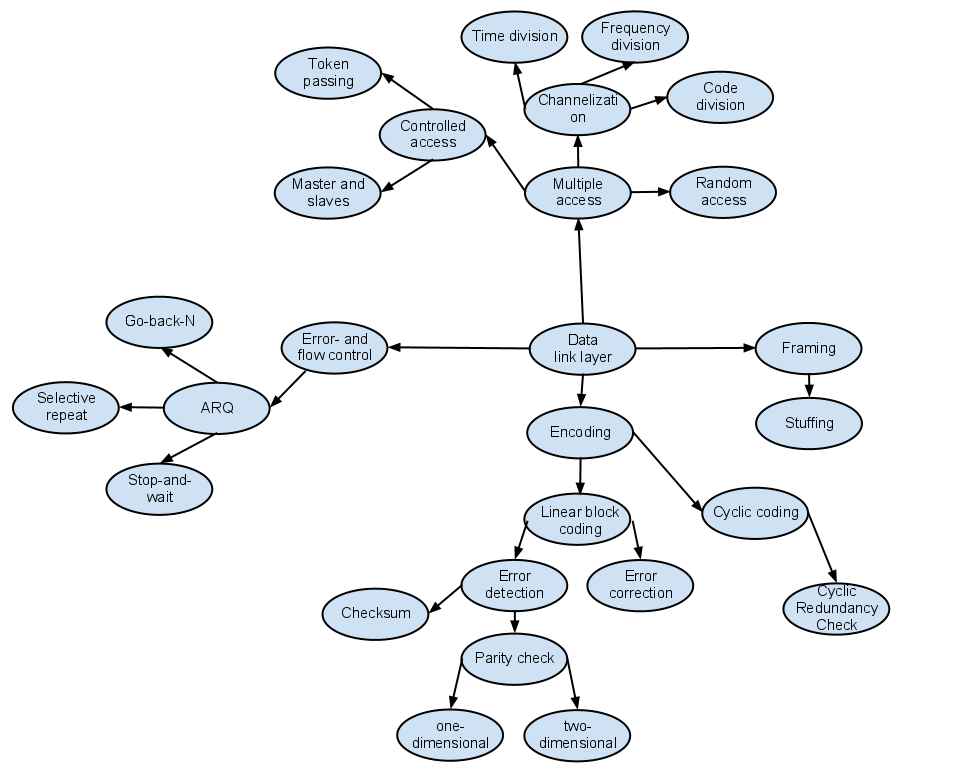
\includegraphics[scale=0.4,trim=0 0 0 0]{dll_bobler.png}%trim=l b r t
	\caption{Things to consider concerning data link layer}
	\label{fig:dll_bobler}
	\end{center}
\end{figure}

\subsection{Encoding}
First thing to consider is the encoding of signals. Since there are sixteen
different DTMF combinations, each tone can carry four bits.

The only type of error to consider is the situation where a tone is
misinterpreted, which leads to a four bit burst error. Therefore the system
should be designed specifically to detect errors of this type. Since the media
is considered to be very noisy, transmissions should also be kept as short as
possible.

A two dimensional parity check will be able to detect burst errors of the
proposed size, so this is the choice. Implementing the parity check as a
four-by-four matrix will make it possible to transfer two bytes with a frame of
three bytes.

Example: We want to transmit the two bytes 0011 0101 and 0101 1110. The data
link layer puts these in a four by four matrix and calculates the parity bits by
adding the rows and columns: \todo{Refer to table by label}

\begin{table}[htb]
	\begin{center}
	\begin{tabular}{c|c}
	0011 & 0 \\
	0101 & 0 \\
	0101 & 0 \\
	1110 & 1 \\
	\hline
	1101 & \\
	\end{tabular}
	\end{center}
	\caption{Two-dimensional parity check}
	\label{tab:two_dimensional_parity_check}
\end{table}

Instead of as normally done to increase the size of each row by one to contain
the parity bit, the parity bits are transmitted together as a redundant byte. In
the case of this example the transmission would be: \todo{Refer to table by label}

\begin{table}[htb]
	\begin{center}
	\begin{tabular}{c|c|c|c|c|c}
	0011 & 0101 & 0101 & 1110 & 0001 & 1101 \\
	\end{tabular}
	\end{center}
	\caption{Bytes to be transmitted}
	\label{tab:bytes_to_be_transmitted}
\end{table}

Each four bit nipple is now transmitted an a DTMF-tone. Should one of the tones
be misinterpreted, the receiving data link layer would get a mismatch of the
parity bits for example:

\begin{table}[htb]
	\begin{center}
	\begin{tabular}{c|c}
	0011 & 0 \\
	0101 & 0 \\
	0000 & 0 \\
	1110 & 1 \\
	\hline
	1000 & \\
	\end{tabular}
	\end{center}
	\caption{Failed parity check}
	\label{tab:failed_parity_check}
\end{table}

This will lead to the frame being discarded. Though in some cases it will be
possible to correct the error and find the original nibble, this is not
recommended, since more than one tone might be corrupted. Errors in the
redundant byte \todo{Ved vi hvilken byte, fejlen er i?} will also lead to the discarding of the transmission.

\subsection{Flow control}
The next thing to consider is flow control. Since the DTMF-system
cannot be used as full-duplex, piggybacking is impossible. This means that at
some point the receiver must reply. This reply will also be of six-tones, and
therefore it might as well contain information about witch frames to resend. In
other words a selective repeat system is preferred

To introduce a selective repeat system, additional redundancy is needed.

By using three bits for the sequence number, redundancy is kept as low as
possible while still benefiting from pipelining. The sender transmits eight
frames (fourty eight tones) and then waits for the receiver to reply with one
frame (six tones).

\subsection{Framing}
It is presumed that the physical layer will provide a starting point for each
transmission. If this is not the case, 
additional flags will be needed in between the frames, \todo{Det m� vi hellere f� styr p� s�} again leading to the need
of stuffing.

Next thing to consider is multipoint. There are three options: \todo{Vi regner med at l�seren kender disse typer, men det er m�ske ogs� i orden} A token
network, a time division network or a code division network. Time division
requires a level of timing the interface layer is unable to deliver.
Code division leads to the need for larger frames or if implemented with the
proposed frame size, a lot of unused frames in a small network. This leaves us
with a token passing network, so this is the choice.

Three bits will control the addressing, all identifying the receiver, since info
about sender is not needed at this level. Thereby the protocol allows networks
of up to eight stations. \todo{Er det statiske addresser eller kan vi v�lge dem gennem backbone/API?}

The selective repeat system and the token network introduces the need for different frame types.
The type field will consist of two bits, at the same time controlling
the token and indicating frame types. Rules must be implemented to keep the token circulating.

\begin{table}[htb]
	\begin{center}
	\begin{tabular}{|c|ll|}
		\multicolumn{1}{c}{\textit{Type}} & \multicolumn{1}{l}{} & \multicolumn{1}{l}{}\\ %''abusing'' \multicolumn to avoid borders
		\hline
		00 & Has no token & Reply from receiver \\
		\hline
		01 & Has no token & Passes token to addressed station \\
		\hline
		10 & Has token & Accepts token from addressed station \\
		\hline
		11 & Has token & Data frame for addressed station \\
		\hline
	\end{tabular}
	\end{center}
	\caption{Protocol for type field}
	\label{tab:protocol_for_type_field}
\end{table}

\todo{Table ref?}
Reply frames has type 00 and sequence number 111 (to prevent legal 0:0:0
frames). Each bit of the data byte corresponds to a sequence number and has
value 1 for accepted and 0 for resend.

Token passing is controlled by the backbone architecture of the system and is
implemented in the data link layer. When the token is offered,
there is a window of response time, wherein the station must reply by accepting
the token. If there are no reply during the window, the token is offered to the
next station. 

The backbone has a routine for asking the data link layer whether
it has the token or not. If there are data to send, this is initialized by the
backbone, else the token is passed to the next station. These functionalities
are implemented as public methods in the data link layer.

This leads to the following format of a frame: 

\begin{table}[htb]
	\begin{center}
	\begin{tabular}{|ccc|c|c|}
		\hline
		type (2 bits) & address (3 bits) & sequence (3 bits) & data (8 bits) & parity
		(8 bits)  \\
		\hline
	\end{tabular}
	\end{center}
	\caption{Final frame format}
	\label{tab:final_frame_format}
\end{table}